\section{Experimental Studies}
\label{sec:experiment}
We examine the difference in the operation of NSGAII and NOSSGA and evaluate their performance with respect to three existing methods (ASTRAL, MP-EST and STELAR). ASTRAL and MP-EST are two of the most widely used and accurate summary methods~\cite{islam2019stelar}. We used three simulated datasets: 10-taxon (\#estimated gene tree: 200)~\cite{bayzid2015weighted}, 11-taxon (\#estimated gene tree: 50)~\cite{chung2011comparing} and 15-taxon (\#estimated gene tree: 100)~\cite{statistical-binning}. Each of them has 10 replicates (R1 to R10). We used False Negative (FN) rate~\cite{bayzid2013naive} to measure the accuracy of the estimated species tree. FN rate expresses the fraction of edges present in the true species tree\footnote{Provided with the dataset} but missing in the estimated tree. %previously studied

We ran the exact version of ASTRAL and STELAR, which are guaranteed to return the globally optimal tree. And we ran MP-EST with 10 random starting points and selected the species tree with the best PL value. For NSGAII and NOSSGA, we carried out 15 independent runs.  

\begin{figure}
	\begin{adjustwidth}{-4cm}{-3cm}
		\centering    
		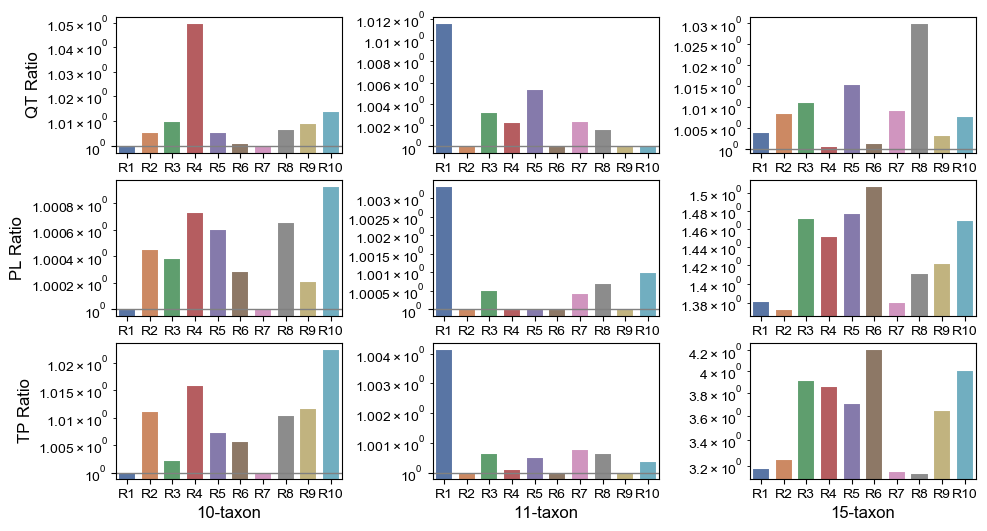
\includegraphics[width=1.6\textwidth]{Figure/tool_ratio}
	\end{adjustwidth}
	\caption{The issue of overshooting the optimization criterion beyond the true tree by existing methods. Each row shows the ratio of scores (QT/PL/TP), optimized by a particular method (ASTRAL/MP-EST/STELAR), of the true tree to that of the estimated tree by the same method.} \label{fig:tool_ratio}
	
\end{figure}

\subsection{Observation}
\label{subsec:observation}
At first, we present an important observation that essentially motivated us to tackle the problem of species tree estimation as a MOP. We mentioned in Section~\ref{sec:intro} that, due to limitation in available knowledge and error introduced in data pre-processing, existing methods may overshoot the criterion they try to optimize, and thus deviate from the true tree. In Fig.~\ref{fig:tool_ratio}, we summarize our observations for three methods (ASTRAL, MP-EST and STELAR) on 10 replicates of our selected datasets. Here, the top row shows the ratio of quartet-scores (QT) of the true trees to quartet-scores (QT) of the ASTRAL-estimated trees. Likewise, the middle row shows the pseudo-likelihood (PL) ratio of the true trees and MP-EST estimated trees and the bottom row does the same with the triplet (TP) ratio of STELAR. As we treat each objective as a minimization form, ideally these ratios should be 1 (marked as a gray horizontal line in each plot). However, we find that in most of the cases the ratio is greater than 1. %And for 15-taxon (third column of Fig.~\ref{fig:tool_ratio}), we 


\subsection{NSGAII vs. NOSSGA}
Now we closely inspect the behavioral difference between NSGAII and NOSSGA to know whether NOSSGA posses our desired properties. We ensured a level playing ground by executing both algorithms with the same configuration (independent run: 15, population size: 100, maximum generations: 99, crossover rate: 0.3, mutation rate: 1.0). For NOSSGA, we use tournament size 10.

\begin{figure}[!htbp]
	%\scriptsize
	\centering
	\begin{adjustwidth}{-1cm}{-1cm}
		\begin{subfigure}[b]{0.4\textwidth}
			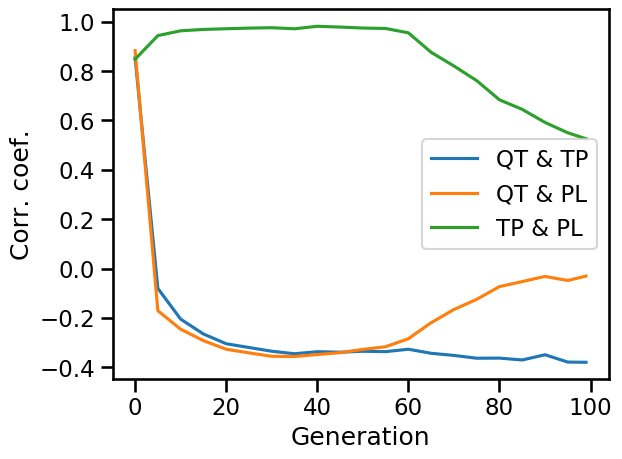
\includegraphics[width=\textwidth]{Figure/10-taxon_NSGAII_corr_plot}
			\caption{NSGAII: 10-taxon}
			%\label{fig:con_pr06}
		\end{subfigure}%
		\begin{subfigure}[b]{0.4\textwidth}
			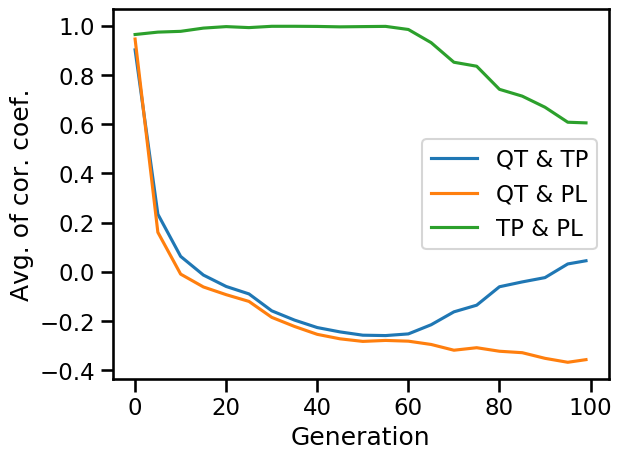
\includegraphics[width=\textwidth]{Figure/11-taxon_NSGAII_corr_plot}
			\caption{NSGAII: 11-taxon}
			%\label{fig:con_pr07}
		\end{subfigure}%
		\begin{subfigure}[b]{0.4\textwidth}
			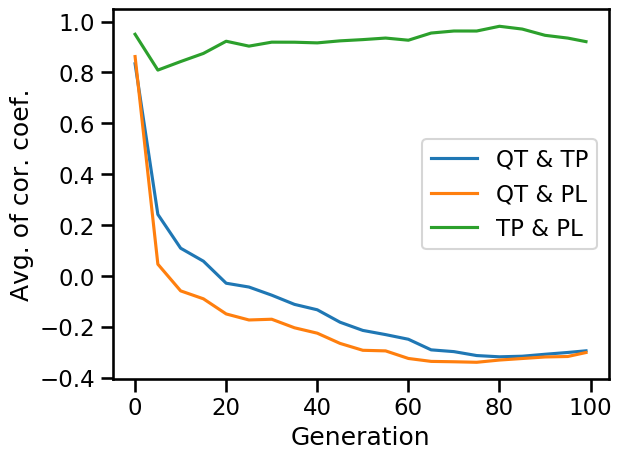
\includegraphics[width=\textwidth]{Figure/15-taxon_NSGAII_corr_plot}
			\caption{NSGAII: 15-taxon}
			%\label{fig:con_pr09}
		\end{subfigure}    
		\begin{subfigure}[b]{0.4\textwidth}
			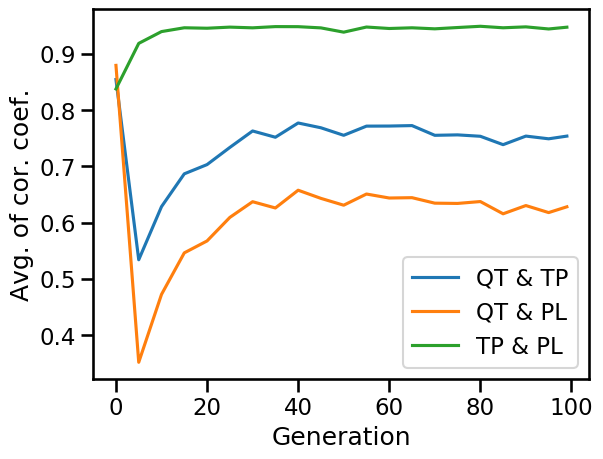
\includegraphics[width=\textwidth]{Figure/10-taxon_NOSSGA_corr_plot}
			\caption{NOSSGA: 10-taxon}
			%\label{fig:con_pr06}
		\end{subfigure}%
		\begin{subfigure}[b]{0.4\textwidth}
			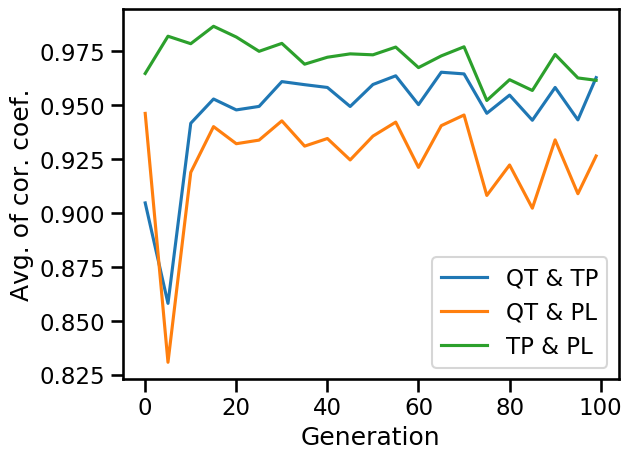
\includegraphics[width=\textwidth]{Figure/11-taxon_NOSSGA_corr_plot}
			\caption{NOSSGA: 11-taxon}
			%\label{fig:con_pr07}
		\end{subfigure}%
		\begin{subfigure}[b]{0.4\textwidth}
			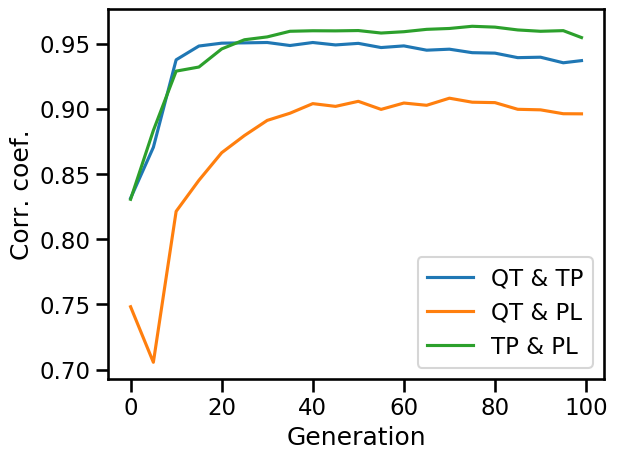
\includegraphics[width=\textwidth]{Figure/15-taxon_NOSSGA_corr_plot}
			\caption{NOSSGA: 15-taxon}
			%\label{fig:con_pr09}
		\end{subfigure}
		\caption{Variation of correlation between each pair of objectives with generations for NSGAII and NOSSGA on three datasets. 
			%The plotted correlation coefficients are averaged over 15 runs and 10 replicates. 
			%In each plot (algorithm: dataset), the correlation coefficient of each point are averaged over 15 runs and 10 replicates.
		}
		\label{fig:gen_wise_correlation}
	\end{adjustwidth}
\end{figure}

\subsubsection{Correlation between two objectives:} We show the variation of correlation between each pair of objectives with generations for NSGAII and NOSSGA on three datasets in Fig.~\ref{fig:gen_wise_correlation}. Here the horizontal axis represents the generations and the vertical axis represents the correlation coefficients averaged over 15 runs and 10 replicates. We see that, contrary to NSGAII, NOSSGA is able to restrict each pair of objectives to be conflicting during the whole period. These results prove that NOSSGA prevents the optimization of one objective to a great extent even at the loss of some other objectives as an attempt to resolve issue~\ref{item:i1}\footnote{Mentioned in Section~\ref{sec:problem}} as we discussed earlier in Section~\ref{sec:method}). %objective to a great extent according to our requirement\footnote{Nayeem link it to the method section in algo}. 

\begin{figure}[!htbp]
	\centering
	\begin{adjustwidth}{-1cm}{-1cm}
		\begin{subfigure}[b]{0.4\textwidth}
			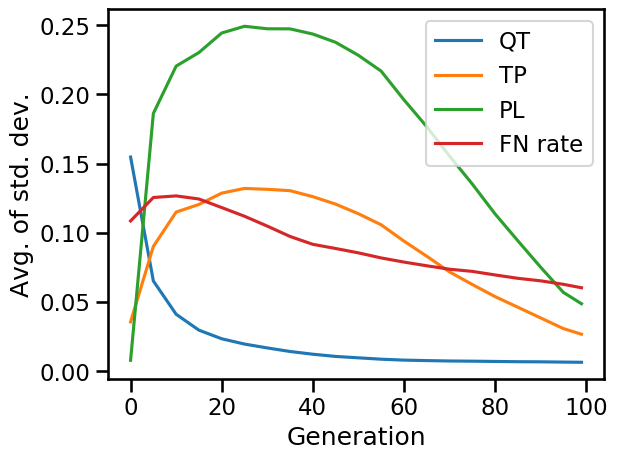
\includegraphics[width=\textwidth]{Figure/10-taxon_NSGAII_std_dev}
			\caption{NSGAII: 10-taxon}
			%\label{fig:con_pr06}
		\end{subfigure}%
		\begin{subfigure}[b]{0.4\textwidth}
			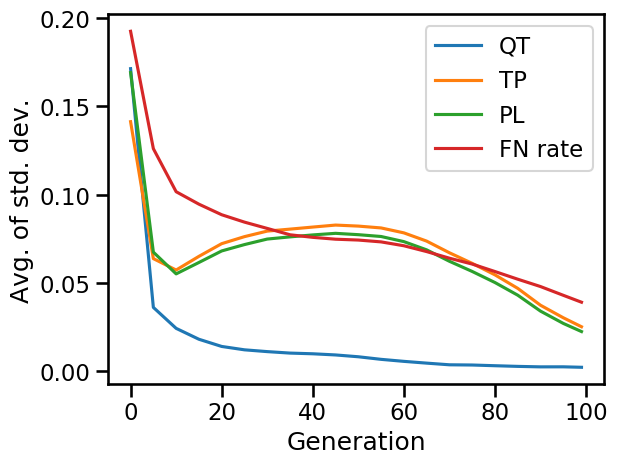
\includegraphics[width=\textwidth]{Figure/11-taxon_NSGAII_std_dev}
			\caption{NSGAII: 11-taxon}
			%\label{fig:con_pr07}
		\end{subfigure}%
		\begin{subfigure}[b]{0.4\textwidth}
			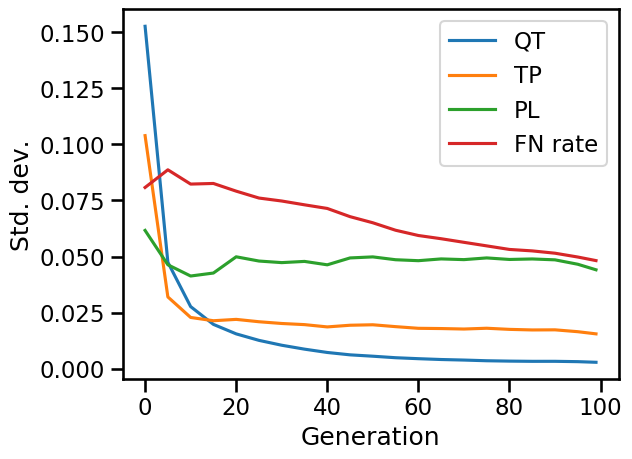
\includegraphics[width=\textwidth]{Figure/15-taxon_NSGAII_std_dev}
			\caption{NSGAII: 15-taxon}
			%\label{fig:con_pr09}
		\end{subfigure}
		\begin{subfigure}[b]{0.4\textwidth}
			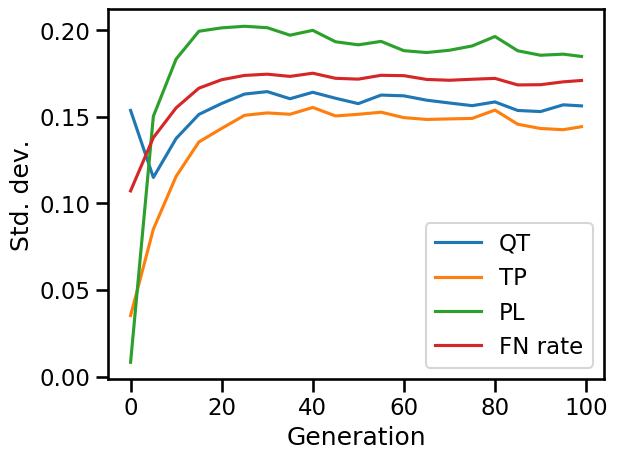
\includegraphics[width=\textwidth]{Figure/10-taxon_NOSSGA_std_dev}
			\caption{NOSSGA: 10-taxon}
			%\label{fig:con_pr06}
		\end{subfigure}%
		\begin{subfigure}[b]{0.4\textwidth}
			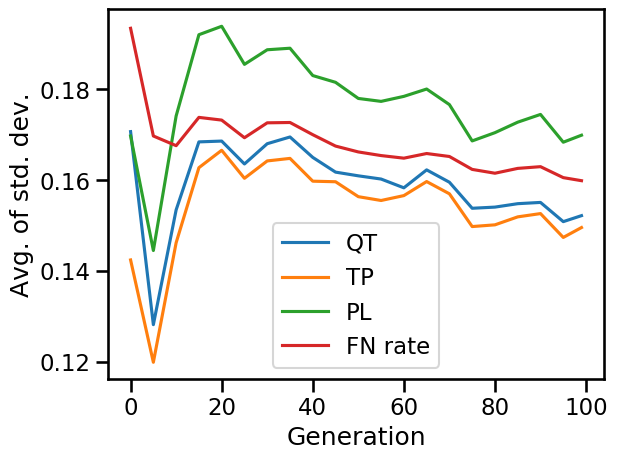
\includegraphics[width=\textwidth]{Figure/11-taxon_NOSSGA_std_dev}
			\caption{NOSSGA: 11-taxon}
			%\label{fig:con_pr07}
		\end{subfigure}%
		\begin{subfigure}[b]{0.4\textwidth}
			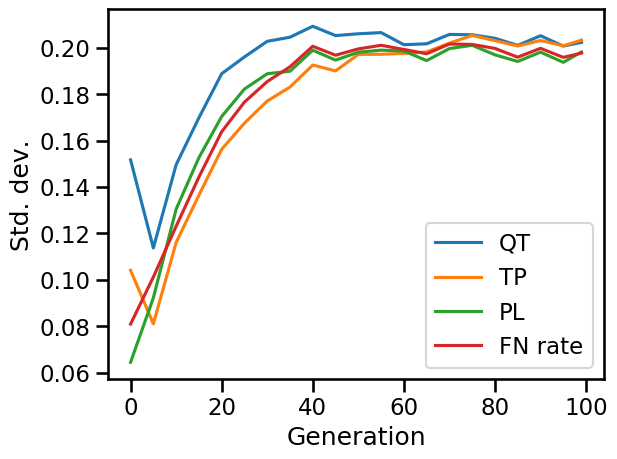
\includegraphics[width=\textwidth]{Figure/15-taxon_NOSSGA_std_dev}
			\caption{NOSSGA: 15-taxon}
			%\label{fig:con_pr09}
		\end{subfigure}
		\caption{Variation of standard deviation of three objectives and FN rates in the population with generations for NSGAII and NOSSGA on three datasets.
			% on three datasets. The plotted standard deviations are averaged over 15 runs and 10 replicates. 
		}
		\label{fig:gen_wise_std_dev}
	\end{adjustwidth}
\end{figure}

\subsubsection{Diversity of objectives and FN rate:}\label{subsubsec:diversity} Fig.~\ref{fig:gen_wise_std_dev} shows the variation of the standard deviation of three objective values\footnote{Normalized using global maximum and minimum.} of the population members and their respective FN rates\footnote{The knowledge of FN rate is absent to the EMOs.} in the population with generations for NSGAII and NOSSGA on three datasets. Along the vertical axis, we plotted the standard deviation values averaged over 15 runs and 10 replicates. These figures clearly show that NSGAII loses diversity at an early stage possibly. This an outcome of not taking necessary measures to tackle issue~\ref{item:i2}~\cite{qu2010multi}.    

\begin{figure}[!htbp]
	\centering
	\begin{adjustwidth}{-1cm}{-1cm}
		\begin{subfigure}[b]{0.4\textwidth}
			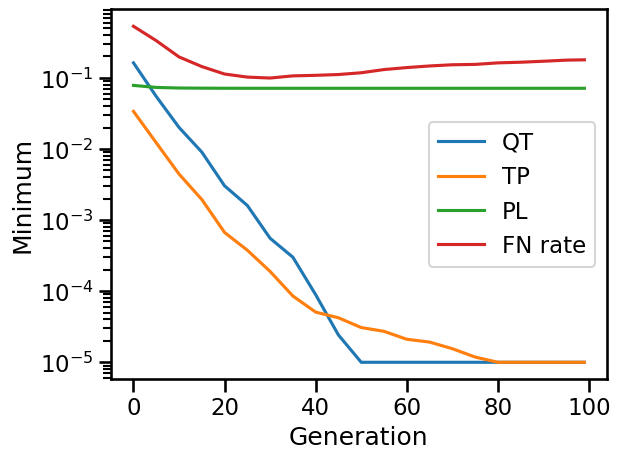
\includegraphics[width=\textwidth]{Figure/10-taxon_NSGAII_minimum}
			\caption{NSGAII: 10-taxon}
			%\label{fig:con_pr06}
		\end{subfigure}%
		\begin{subfigure}[b]{0.4\textwidth}
			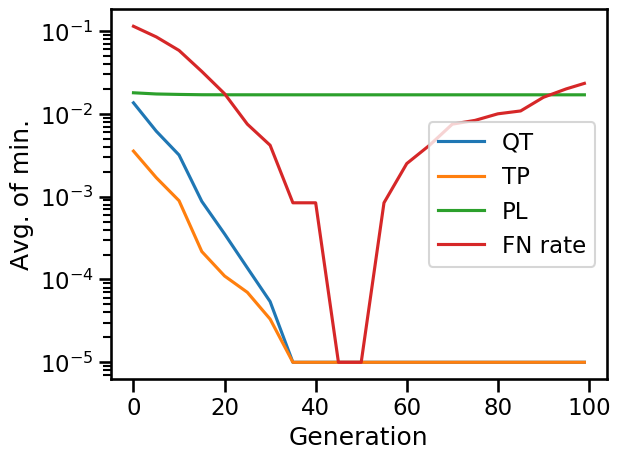
\includegraphics[width=\textwidth]{Figure/11-taxon_NSGAII_minimum}
			\caption{NSGAII: 11-taxon}
			%\label{fig:con_pr07}
		\end{subfigure}%
		\begin{subfigure}[b]{0.4\textwidth}
			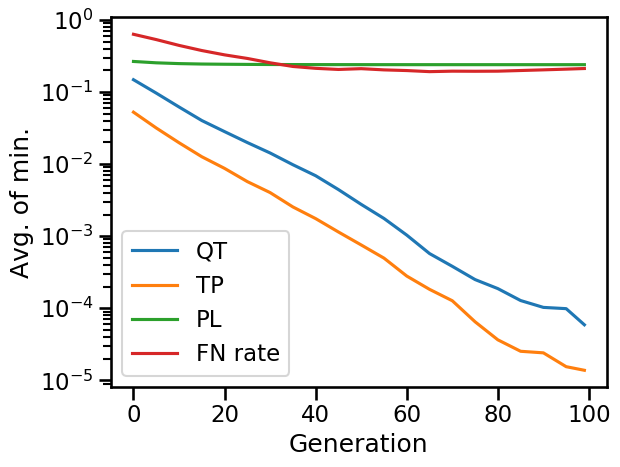
\includegraphics[width=\textwidth]{Figure/15-taxon_NSGAII_minimum}
			\caption{NSGAII: 15-taxon}
			%\label{fig:con_pr09}
		\end{subfigure}
		\begin{subfigure}[b]{0.4\textwidth}
			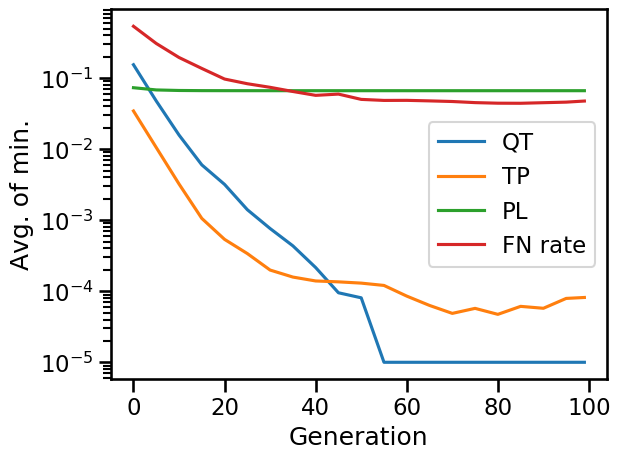
\includegraphics[width=\textwidth]{Figure/10-taxon_NOSSGA_minimum}
			\caption{NOSSGA: 10-taxon}
			%\label{fig:con_pr06}
		\end{subfigure}%
		\begin{subfigure}[b]{0.4\textwidth}
			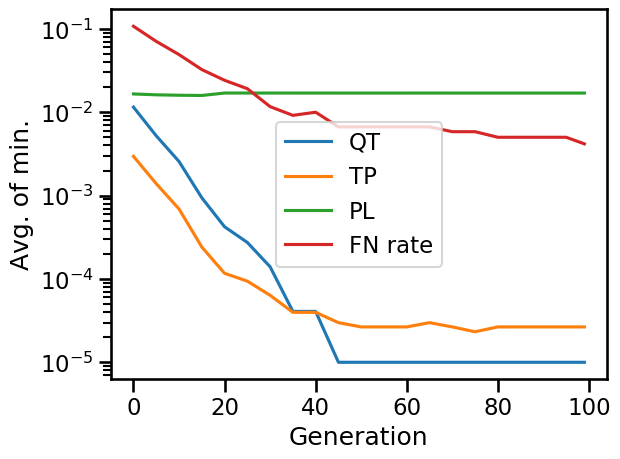
\includegraphics[width=\textwidth]{Figure/11-taxon_NOSSGA_minimum}
			\caption{NOSSGA: 11-taxon}
			%\label{fig:con_pr07}
		\end{subfigure}%
		\begin{subfigure}[b]{0.4\textwidth}
			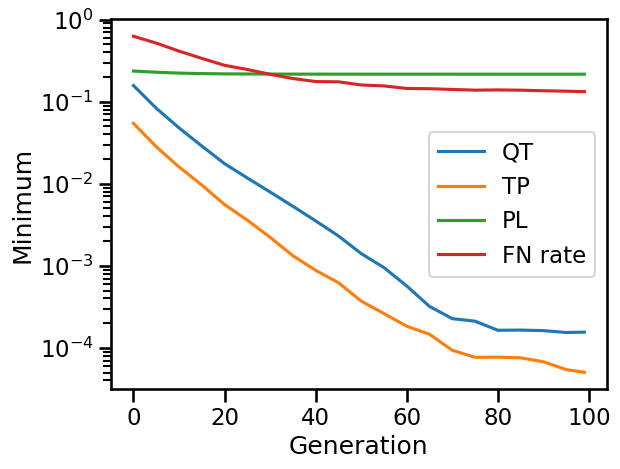
\includegraphics[width=\textwidth]{Figure/15-taxon_NOSSGA_minimum}
			\caption{NOSSGA: 15-taxon}
			%\label{fig:con_pr09}
		\end{subfigure}
		\caption{Variation of minimum of three objectives and FN rates in the population with generations for NSGAII and NOSSGA on three datasets.
			%The plotted minimum values are averaged over 15 runs and 10 replicates. 
		}
		\label{fig:gen_wise_min}
	\end{adjustwidth}
\end{figure}

\subsubsection{Improvement in objectives and FN rate:} Now we observe how the best (minimum) value of three objectives\footnote{We treated each objective as a minimization} and FN rate\footnote{Lower is better} in the population improves across generations for NSGAII and NOSSGA as depicted in Fig.~\ref{fig:gen_wise_min}. The plotted minimum values are averaged over 15 runs and 10 replicates. NSGAII allows one or more objectives to improve as much as possible which causes the resultant species tree to deviate from the true tree (issue~\ref{item:i1}). As a result, the best FN rate of NSGAII starts to degrade after a particular generation. On the other hand, to avoid such deviation, NOSGGA restricts the improvement of one or more objectives after a certain generation. So its FN rate continues to improve. From these results, we can see that NOSSGA is more effective than NSGAII in dealing issue~\ref{item:i1}.%(except PL\footnote{To decrease the large runtime of PL calculation using MP-EST, we decreased the default iteration count})

\begin{figure}[!htbp]
	\centering
	\begin{adjustwidth}{-1cm}{-1cm}
		\begin{subfigure}[b]{0.4\textwidth}
			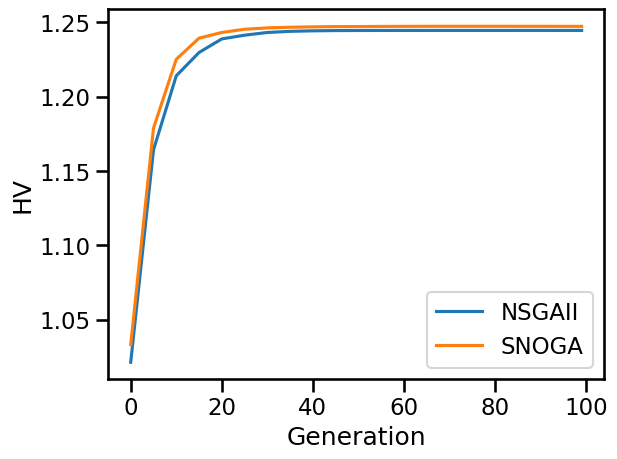
\includegraphics[width=\textwidth]{Figure/10-taxon_hv}
			\caption{10-taxon}
			%\label{fig:con_pr06}
		\end{subfigure}%
		\begin{subfigure}[b]{0.4\textwidth}
			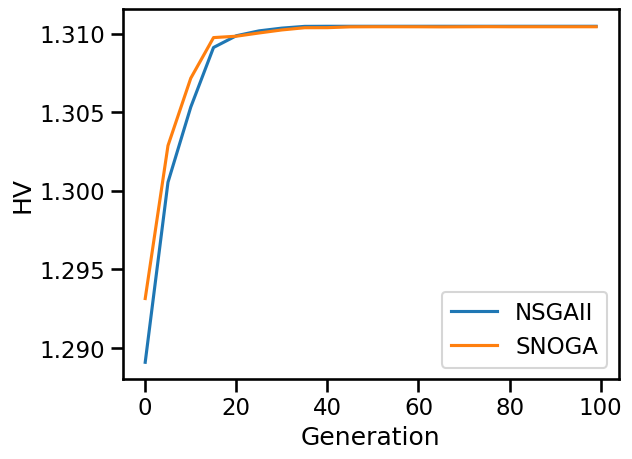
\includegraphics[width=\textwidth]{Figure/11-taxon_hv}
			\caption{11-taxon}
			%\label{fig:con_pr07}
		\end{subfigure}%
		\begin{subfigure}[b]{0.4\textwidth}
			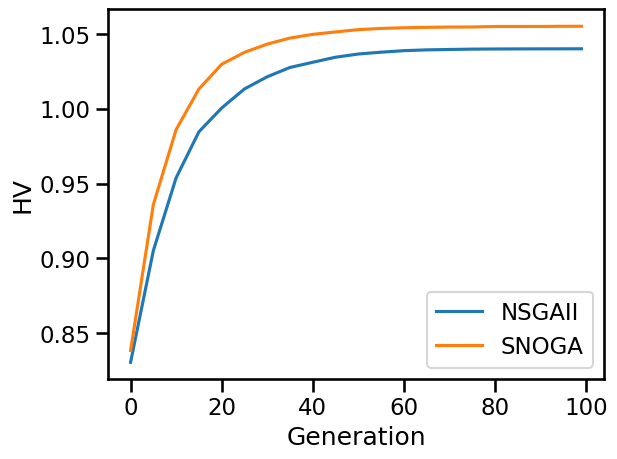
\includegraphics[width=\textwidth]{Figure/15-taxon_hv}
			\caption{15-taxon}
			%\label{fig:con_pr09}
		\end{subfigure}
		\caption{Variation of HV with generations for NSGAII and NOSSGA on three datasets.}
		\label{fig:gen_wise_hv}
	\end{adjustwidth}
\end{figure}

\subsubsection{Comparison based on hypervolume:} We mentioned in Section~\ref{sec:problem} that the problem that we deal with in this paper is different from the traditional MOPs. Importantly, the definition of convergence for MOPs is not exactly the same as the convergence within the context of this problem. To explore this issue, we compare NSGAII and NOSSGA in terms of hypervolume (HV)~\cite{zitzler1999multiobjective} which is probably the most popular performance measure used for MOPs. HV captures both convergence and diversity of the PF, sampled by an EMO algorithm, in a single real-value. For MOPs with all minimization objectives, a higher value of HV is desirable. In Fig.~\ref{fig:gen_wise_hv}, we plot the HV values averaged over 15 runs and 10 replicates. From these results, it is difficult to differentiate between these two algorithms. Both of their HV values get saturated at an early generation. Interestingly, according to HV, NOSSGA seems better than NSGAII. This is probably due to the loss of diversity at an early stage as we saw earlier. 

\begin{figure}
	\centering
	\begin{adjustwidth}{-2cm}{-2cm}
		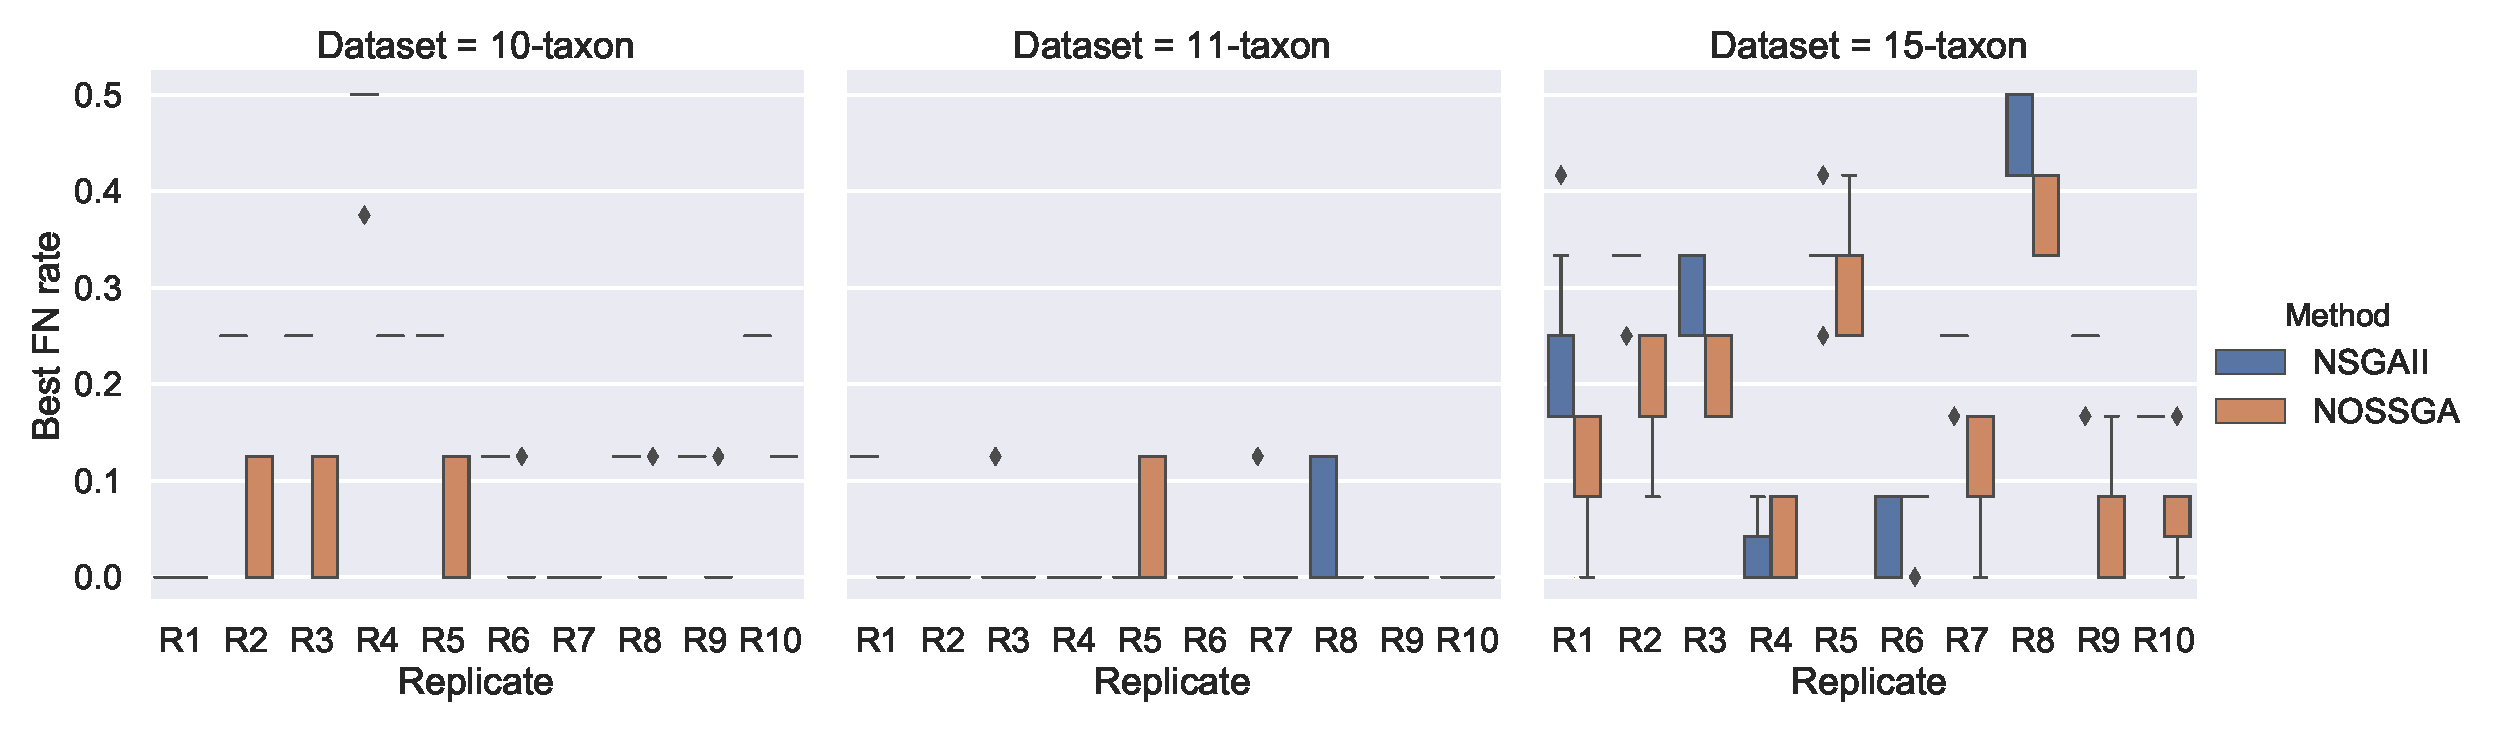
\includegraphics[width=1.5\textwidth]{Figure/emo_boxplot}
		\caption{Accuracy of the best estimated species trees extracted from the final population of NSGAII and NOSSGA on each dataset having 10 replicate.} \label{fig:emo_compare}
	\end{adjustwidth}
\end{figure}

\subsubsection{Comparison based on Tree accuracy:} Finally we compare NSGAII and NOSSGA in terms of the tree accuracy for 10 replicates of each dataset. So we graphically summarize the FN rate (lower value means more accurate) of the best trees from the final population of 15 independent runs using boxplots in Fig.~\ref{fig:emo_compare}. We observe that NOSSGA can offer much better solutions than NSGAII in most of the cases. In a few situations, two algorithms perform equally.

\begin{figure}
	\begin{adjustwidth}{0cm}{0cm}
		\centering
		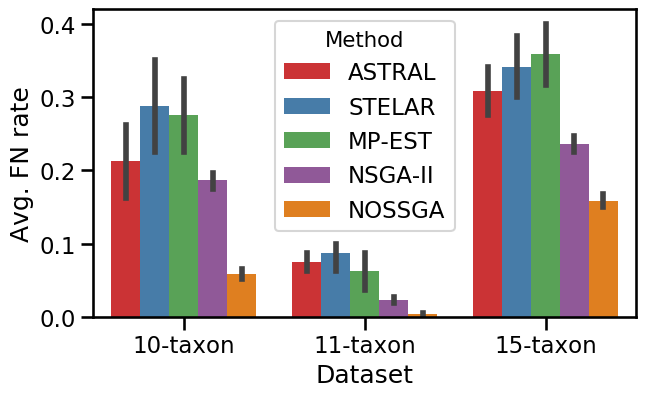
\includegraphics[width=0.8\textwidth]{Figure/all_dataset_compare}
		\caption{Performance comparison of ASTRAL, STELAR, MP-EST, NSGAII and NOSSGA on three datasets. 
			%We show the average FN rates with standard error bars over 10 replicates
		} \label{fig:compare_exisitng_methods}
	\end{adjustwidth}
\end{figure}

\subsection{Comparison with Existing Methods}
We evaluated the best trees offered by NSGAII and NOSSGA in comparison with the output of ASTRAL, MP-EST and STELAR. 
%ASTRAL and MP-EST are two of the most widely used and accurate summary methods. We ran the exact version of ASTRAL and STELAR, which are guaranteed to return the globally optimal tree. And for MP-EST, we ran with 10 random starting points and selected the species tree with the highest PL value. 
On each dataset, we ran both NSGAII and NOSSGA only for 99 generations (population size: 100, function evaluations: 10000). 
Fig.~\ref{fig:compare_exisitng_methods} shows the average FN rates with standard error bars over 10 replicates. We find that NOSSGA offers the highest accuracy among all. On the 10-taxon dataset, NOSSGA can achieve nearly 4X accuracy than ASTRAL. For the rest two datasets, the accuracy improvement is around 2X compared to ASTRAL. Interestingly, even the basic NSGAII exhibits more accuracy than the three existing methods. So the advantage of formulating this problem as a MOP is obvious. However, if we run the basic NSGAII for a large number of generations its accuracy may fall for not resolving the issues mentioned in Section~\ref{sec:problem} properly which we saw earlier. So we can state that, owing to the characteristics designed considering the problem nature, NOSSGA achieves at least 1.4X accuracy gain over the basic NSGAII in all cases. 



%\subsection{Discussion}

\begin{comment}
\begin{figure}[!htbp]
\centering
\begin{adjustwidth}{-1cm}{}
\begin{subfigure}[b]{0.55\textwidth}
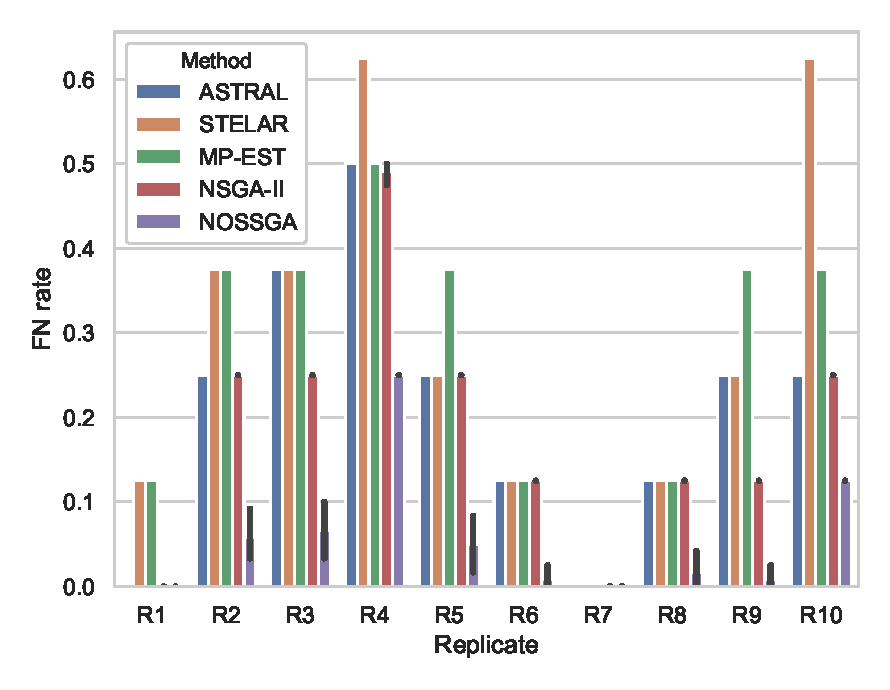
\includegraphics[width=\textwidth]{Figure/10-taxon_10_replicates}
\caption{10-taxon}
%\label{fig:con_pr06}
\end{subfigure}%
\begin{subfigure}[b]{0.55\textwidth}
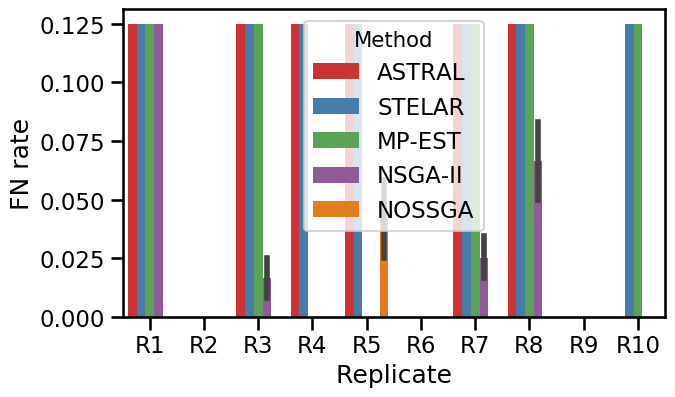
\includegraphics[width=\textwidth]{Figure/11-taxon_10_replicates}
\caption{11-taxon}
%\label{fig:con_pr07}
\end{subfigure}%
%    \newline

\begin{subfigure}[b]{0.55\textwidth}
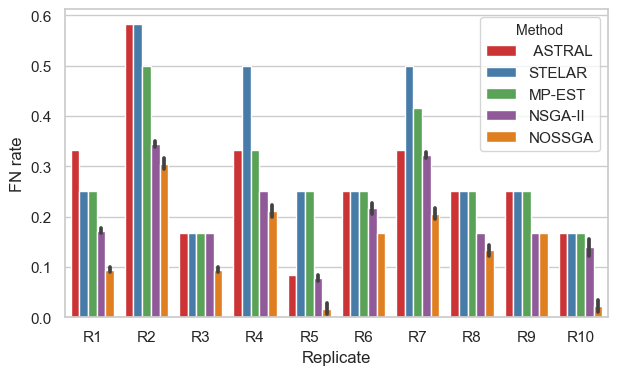
\includegraphics[width=\textwidth]{Figure/15-taxon_10_replicates}
\caption{15-taxon}
%\label{fig:con_pr09}
\end{subfigure}
\begin{subfigure}[b]{0.55\textwidth}
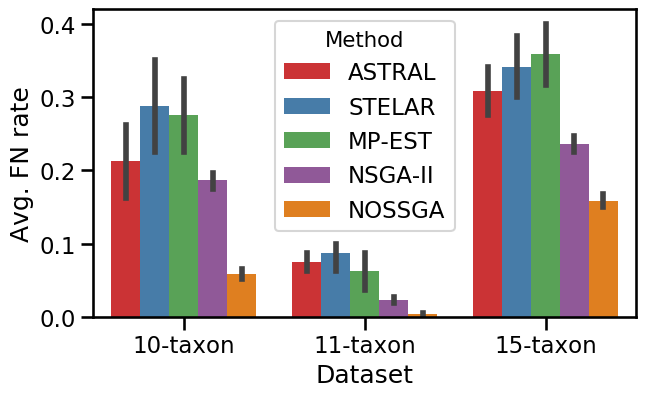
\includegraphics[width=\textwidth]{Figure/all_dataset_compare}
\caption{Summary}
%\label{fig:con_pr09}
\end{subfigure}%

\caption{Comparison of ASTRAL, STELAR, MP-EST, NSGAII and NOSSGA on 10 replicates of 3 datasets.}
\label{fig:datasets}
\end{adjustwidth}
\end{figure}



\begin{figure}[!htbp]
\centering
\begin{adjustwidth}{-1cm}{}
\begin{subfigure}[b]{0.48\textwidth}
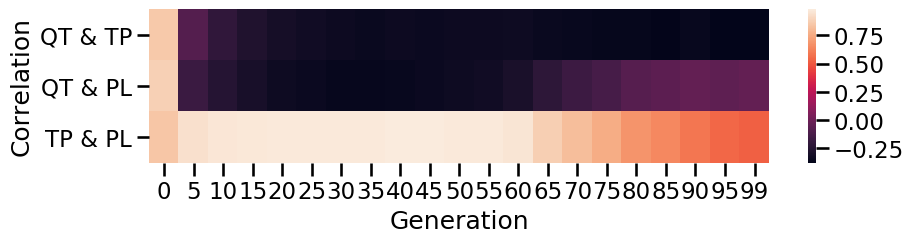
\includegraphics[width=\textwidth]{Figure/10-taxon_NSGA-II_heatmap}
\caption{NSGAII: 10-taxon}
%\label{fig:con_pr06}
\end{subfigure}%
\begin{subfigure}[b]{0.4\textwidth}
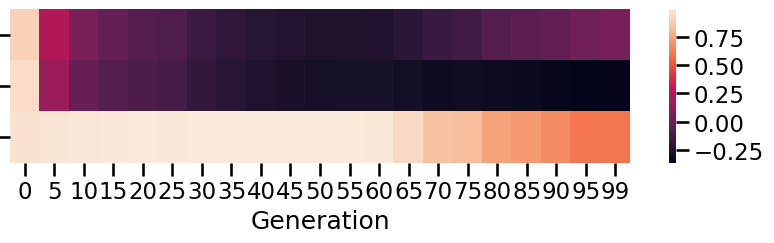
\includegraphics[width=\textwidth]{Figure/11-taxon_NSGA-II_heatmap}
\caption{NSGAII: 11-taxon}
%\label{fig:con_pr07}
\end{subfigure}%
\begin{subfigure}[b]{0.4\textwidth}
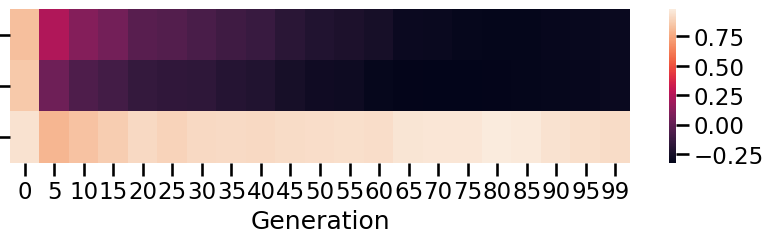
\includegraphics[width=\textwidth]{Figure/15-taxon_NSGA-II_heatmap}
\caption{NSGAII: 15-taxon}
%\label{fig:con_pr09}
\end{subfigure}

\begin{subfigure}[b]{0.48\textwidth}
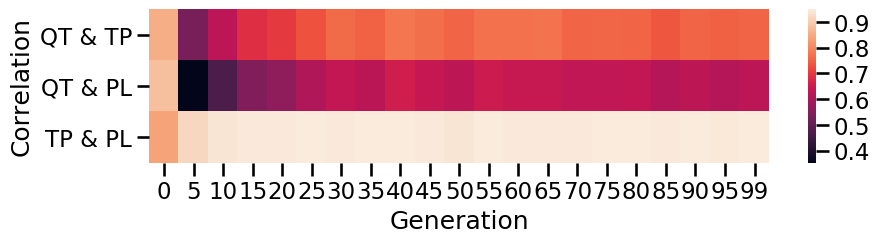
\includegraphics[width=\textwidth]{Figure/10-taxon_NOSSGA_heatmap}
\caption{NOSSGA: 10-taxon}
%\label{fig:con_pr06}
\end{subfigure}%
\begin{subfigure}[b]{0.4\textwidth}
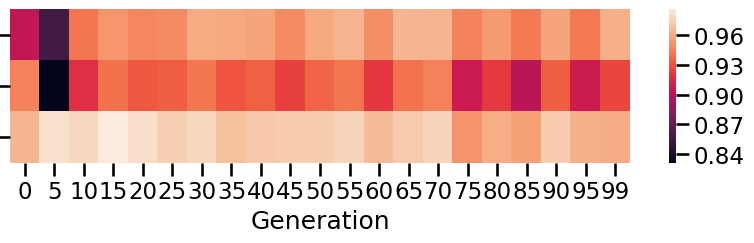
\includegraphics[width=\textwidth]{Figure/11-taxon_NOSSGA_heatmap}
\caption{NOSSGA: 11-taxon}
%\label{fig:con_pr07}
\end{subfigure}%
\begin{subfigure}[b]{0.4\textwidth}
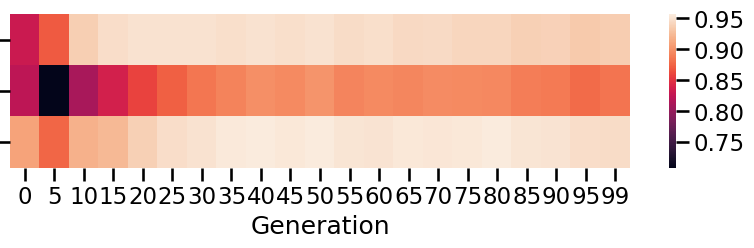
\includegraphics[width=\textwidth]{Figure/15-taxon_NOSSGA_heatmap}
\caption{NOSSGA: 15-taxon}
%\label{fig:con_pr09}
\end{subfigure}
\caption{Correlation between each pair of objectives as the generation of an EMO progresses. For each dataset, we average the correlation coefficient over 15 runs and 10 replicates.}
\label{fig:gen_wise_correlation}
\end{adjustwidth}
\end{figure}
%\begin{figure}
%    \centering
%    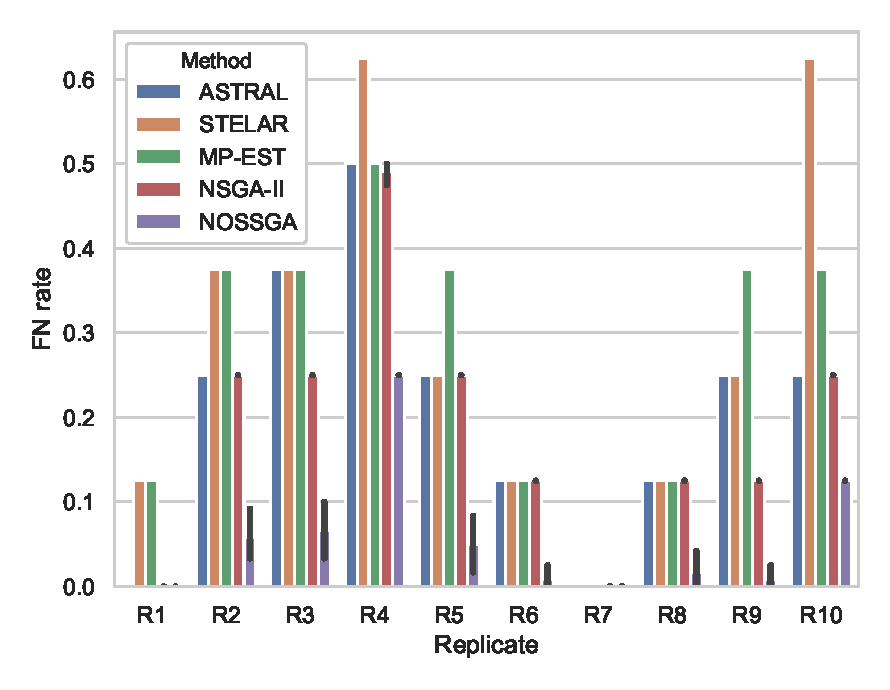
\includegraphics[width=0.6\textwidth]{Figure/10-taxon_10_replicates}
%    \caption{10-taxon.} \label{fig1}
%\end{figure}
%\begin{figure}
%    \centering
%    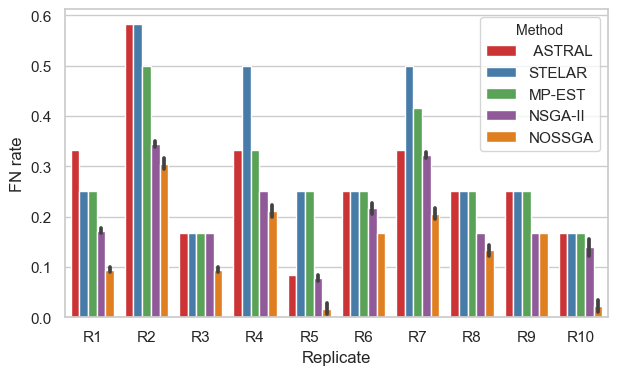
\includegraphics[width=0.6\textwidth]{Figure/15-taxon_10_replicates}
%    \caption{15-taxon.} \label{fig2}
%\end{figure}
\subsection{Results on 10-taxon dataset}
\subsection{Results on 11-taxon dataset}
\subsection{Results on 15-taxon dataset}
\end{comment}

